\documentclass[10pt]{article}
\usepackage{fancyhdr}
\usepackage{listings}
\usepackage{graphicx}

\setlength{\textwidth}{7.25in}
\setlength{\textheight}{9.0in}
\setlength{\topmargin}{-0.75in}
\setlength{\oddsidemargin}{-0.5in}
\setlength{\evensidemargin}{-0.5in}
\setlength{\headheight}{47pt}

\setlength\parindent{0pt}

\fancyhead[R]{CS 111C Jessica Masters\\
				Homework 10\\
				Chapters 25-28 Trees\\
				Richard Szeto}
				
\pagestyle{fancy}

\lstset{language=Java}

\begin{document}

\begin{center}
	\Large{\textbf{Homework 10}}
\end{center}

\section{Chapter 25: Trees}

\begin{enumerate}
	\item[3.] Consider a binary tree that has three levels.
		\begin{enumerate}
			\item What is the maximum number of nodes in this tree?
				
				\vspace{0.5cm}
				If level 1 is the root of the tree, then level 1 has a maximum of 1 node, level 2 has a maximum of 2 nodes, and level 3 has a maximum of 4 nodes. That is a total of 7 nodes in a three level tree. A three level tree also has a height of 3. That means there are $2^3 - 1$ nodes, which is equivalent to 7 nodes.
				\vspace{0.5cm}
			
			\item What is the maximum number of leaves in this tree?
				
				\vspace{0.5cm}
				To have the maximum number of leaves, the tree must be complete. This is because the number of nodes on some level is twice the number of nodes on a previous level. In other words, $N_l = 2 * N_{l - 1}$, where $N$ is the number of nodes, $l$ is the level number, and $N_1 = 1$. Therefore, the maximum number of leaves in three level binary tree is 4. We can do this calculation by subtracting the maximum number of nodes in a two level binary tree from the maximum number of nodes in a three level binary tree. $(2^3 - 1) - (2^2 - 1) = 7 - 3 = 4$
				\vspace{0.5cm}
			
			\item Answer the previous two questions for a binary tree that has ten levels.
				\begin{enumerate}
					\item The maximum number of nodes in a ten level binary tree is $2^{10} - 1 = 1023$.
					
					\item The maximum number of leaves in a ten level binary tree is $(2^{10} - 1) - (2^{9} - 1) = 1023 - 511 = 512$
				\end{enumerate}
		\end{enumerate}
	
	\item[7.] Consider a traversal of a binary tree. Suppose that visiting a node means to simply display the data in the node. What are the results of each of the following traversals of the tree in Figure 25-23b
		\begin{enumerate}
			\item Preorder: 11 8 3 2 1 5 4 6 10 9 7
			
			\item Postorder: 2 1 3 4 6 5 8 9 7 10 11
			
			\item Inorder: 2 3 1 8 4 5 6 11 9 10 7
		\end{enumerate}
	
	\item[8.] The two trees in Figure 25-23 contain integer data.
		\begin{enumerate}
			\item Is the tree in Part \textit{a} a binary search tree? Why or why not?
				
				\vspace{0.5cm}
				25-23a is not a binary search tree because the node that contains the key, 8, violates the definition of a binary search tree. It is not the case that the node that contains 8 as its key is greater than all the data in the node's left subtree, in particular the node that contains 9 as its key.
				\vspace{0.5cm}
			
			\item Is the tree in Part \textit{b} a maxheap? Why or why not?
				
				\vspace{0.5cm}
				25-23b is not a maxheap because the node that contains the key, 5, violates the definition of a maxheap. It is not the case that the node that contains 5, is greater than or equal to its descendant objects, in particular the node that contains 6.
				\vspace{0.5cm}
		\end{enumerate}
	
	\item[9.] Draw the shortest possible binary search tree from the following strings: \textit{Ann, Ben, Chad, Drew, Ella, Jenn, Jess, Kip, Luis, Pat, Rico, Scott, Tracy, Zak}. Is your tree unique?
		\begin{itemize}
			\item The question lists the elements that will go in the tree, \textbf{not} the insertion order.
		\end{itemize}
		
		\vspace{0.5cm}
		A level three tree can contain a maximum of $2^3 - 1 = 7$ nodes, and a level four tree can contain a maximum of $2^4 - 1 = 15$ nodes. Since our tree will have 14 nodes, the shortest tree we can make will be a height of 4. Also, since we will not have a full level four tree, the tree will not be unique.
		\vspace{0.5cm}
		
		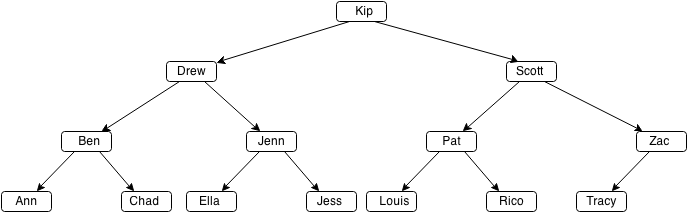
\includegraphics[width=6.5in]{images/25_9.png}
		\vspace{0.5cm}
	
	\item[11.] Draw a maxheap from the strings given in Exercise 9. Is your maxheap unique?
		\begin{itemize}
			\item The question lists the elements that will go in the tree, \textbf{not} the insertion order.
		\end{itemize}
		
		\vspace{0.5cm}
		By the definition of a maxheap, there is no rule that differentiates the left subtree of a node from its right subtree. The data that will be inserted are not all identical to each other, the shortest binary tree will not be full, and the tree will be larger than a level one binary tree. Therefore, the maxheap will not be unique.
		\vspace{0.5cm}
		
		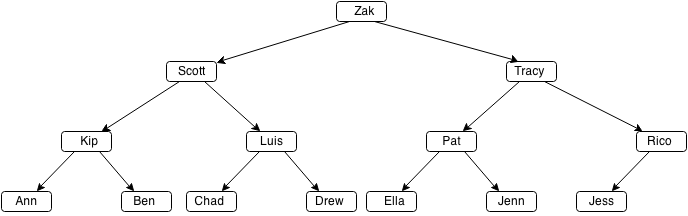
\includegraphics[width=6.5in]{images/25_11.png}
		\vspace{0.5cm}
	
	\item[19.] Draw an expression tree for the algebraic expression $(a + b) * (c - d)$.
		
		\vspace{0.5cm}
		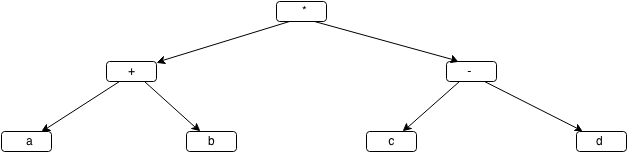
\includegraphics[width=6.5in]{images/25_19.png}
		\vspace{0.5cm}
	
	\item[EC] Suppose we know that the preorder traversal of a binary search tree is 15 10 8 12 11 19 23 21 24. What is the postorder traversal of the tree?
		
		\vspace{0.5cm}
		8 11 12 10 21 24 23 19 15
		\vspace{0.5cm}
\end{enumerate}

\section{Chapter 26: Tree Implementations}

\begin{enumerate}
	\item[7.] Suppose we want to create a method for the class \texttt{BinaryTree} that counts the number of times an object occurs in the tree. The header of the method could be as follows:
		
		\vspace{0.1cm}
		\texttt{public int count(T anObject)}
		\begin{enumerate}
			\item Write this method using a private recursive method of the same name.
				\begin{itemize}
					\item This method would go inside the \texttt{BinaryTree} class. The recursive method should take only two parameters: a \texttt{BinaryNodeInterface<T>} object and an object of type \texttt{T}. The code in segment 26.12 should be helpful.
				\end{itemize}
				
				\vspace{0.5cm}
				Refer to the bottom of BinaryTree.java
				\vspace{0.5cm}
		\end{enumerate}
	
	\item[10.] What binary tree represents the general tree in each of the following figures from the previous chapter?
		\begin{enumerate}
			\item Figure 25-5
				\begin{itemize}
					\item Use the algorithm from the textbook, which is also contained in the online notes. For your answer, draw the binary tree.
				\end{itemize}
				
				\vspace{0.5cm}
				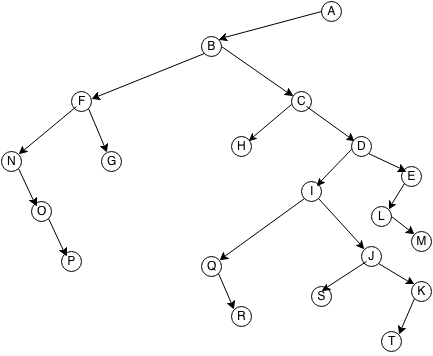
\includegraphics[scale=0.5]{images/26_10.png}
				\vspace{0.5cm}
		\end{enumerate}
	
	\item[12.] Knowing the preorder and inorder traversals of a binary tree will enable you to uniquely define the tree. The same is true for the postorder and inorder traversals.
		\begin{enumerate}
			\item Draw the unique binary tree that has the following preorder and inorder traversals:
				
				\vspace{0.1cm}
				Preorder: A, B, D, E, C, F, G, H
				
				\vspace{0.1cm}
				Inorder: E, D, B, A, G, F, H, C
				
				\vspace{0.5cm}
				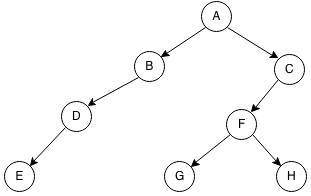
\includegraphics[scale=0.5]{images/26_12.png}
				\vspace{0.5cm}
		\end{enumerate}
	
	\item[13.] Although you can uniquely construct a binary tree from either its preorder and inorder traversals or its postorder and inorder traversals, more than one binary tree can have the same preorder traversal and same postorder traversal. Give an example of two different binary trees with the same preorder and postorder traversals.
	
		\vspace{0.5cm}
		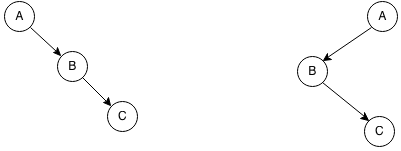
\includegraphics[scale=0.5]{images/26_13.png}
		\vspace{0.5cm}
		
		preorder: A B C
		
		\vspace{0.1cm}
		postorder: C B A
		\vspace{0.5cm}
\end{enumerate}

\section{Chapter 27: Binary Search Tree Implementation}

\begin{enumerate}
	\item[1.] Show the results of adding the following search keys to an initially empty binary search tree: 10, 5, 6, 13, 15, 8, 14, 7, 12, 4.
		\begin{itemize}
			\item The question specifies the insertion order.
		\end{itemize}
		
		\vspace{0.5cm}
		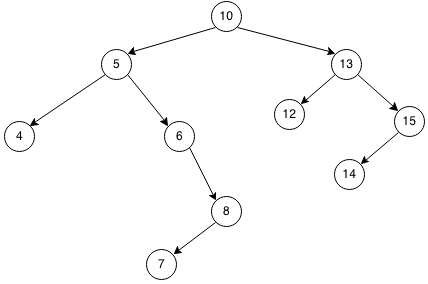
\includegraphics[scale=0.5]{images/27_1.png}
		\vspace{0.5cm}
	
	\item[2.] What ordering of the search keys 10, 5, 6, 13, 15, 8, 14, 7, 12, 4 would result in the most balanced tree if they were added to an initially empty binary search tree?
		\begin{itemize}
			\item For your answer, submit the order \textbf{and} a drawing of the tree. Note that there is more than one right answer.
		\end{itemize}
		
		\vspace{0.5cm}
		Insert order: 12, 7, 5, 4, 6, 10, 8, 14, 13, 15
		
		\vspace{0.5cm}
		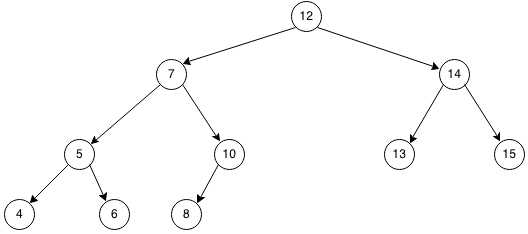
\includegraphics[scale=0.5]{images/27_2.png}
		\vspace{0.5cm}
		
	\item[3.] Give four different orderings of the search keys 10, 5, 6, 13, 15, 8, 14, 7, 12, 4 that would result in the least balanced tree if they were added to an initially empty binary search tree.
		\begin{itemize}
			\item Provide \textbf{three} orderings. For each ordering, submit the order \textbf{and} a drawing of the tree.
		\end{itemize}
		
		\vspace{0.5cm}
		Insert order: 4, 5, 6, 7, 8, 10, 12, 13, 14, 15
		
		\vspace{0.5cm}
		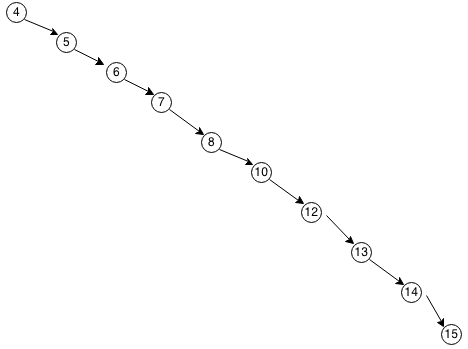
\includegraphics[scale=0.5]{images/27_3_1.png}
		
		\vspace{0.5cm}
		Insert order: 15, 14, 13, 12, 10, 8, 7, 6, 5, 4
		
		\vspace{0.5cm}
		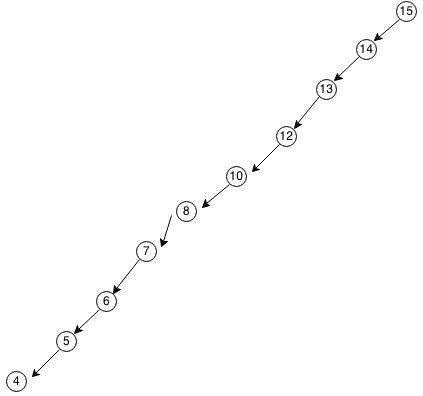
\includegraphics[scale=0.5]{images/27_3_2.png}
		
		\vspace{0.5cm}
		Insert order: 4, 15, 14, 13, 12, 10, 8, 7, 6, 5
		
		\vspace{0.5cm}
		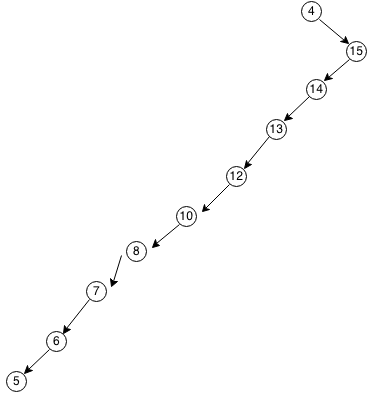
\includegraphics[scale=0.5]{images/27_3_3.png}
		\vspace{0.5cm}
	
	\item[7.] Remove \textit{Doug} from the binary search tree pictured in Figure 27-11d in two different ways.
		
		\vspace{0.5cm}
		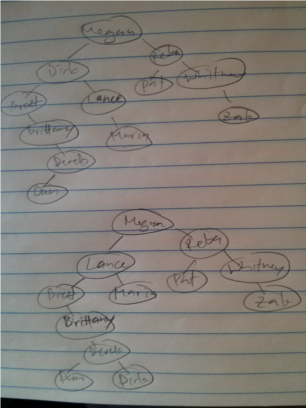
\includegraphics{images/27_7.png}
		\vspace{0.5cm}
	
	\item[15.] Write an algorithm that returns the smallest search key in a binary search tree.
		\begin{itemize}
			\item Pseudocode is fine.
		\end{itemize}
		
		\vspace{0.5cm}
		Note: This code does not use the ADT Dictionary, so the data member in BinaryNode is the key.
		
		\begin{lstlisting}
public T smallestNode()
{
    BinaryNodeInterface<T> currentNode = getRootNode();
    BinaryNodeInterface<T> previousNode = null;

    while(currentNode != null)
    {
        previousNode = currentNode;
        currentNode = currentNode.getLeftChild();
    }
	
	if(previousNode != null)
	    return previousNode.getData();
	
	return null;
}
		\end{lstlisting}
\end{enumerate}

\section{Chapter 28: Heap Implementation}

\begin{enumerate}
	\item[1.] Trace the formation of a maxheap by the constructor given in Segment 28.16 for each of the following arrays:
		\begin{enumerate}
			\item 10 20 30 40 50
				\begin{itemize}
					\item This question asks you to trace the creation of the heap by creating a complete tree and then iteratively using the reheap method - this is the second approach described in the online notes. Show the array \textbf{and} the tree for each step. Show the initial formation of the array/tree and show what the array/tree look like after \textit{each} call to reheap. Remember that reheap is not called for each node when you use this approach to create a heap.
				\end{itemize}
				
				\vspace{0.5cm}
				Original Array: null 10 20 30 40 50
				
				\vspace{0.5cm}
				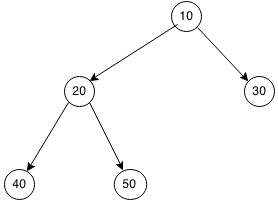
\includegraphics[scale=0.5]{images/28_1_1.png}
				
				\vspace{0.5cm}
				After reheap(2): null 10 50 30 40 20
				
				\vspace{0.5cm}
				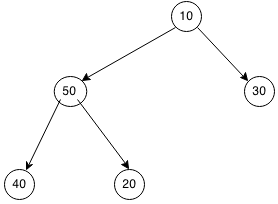
\includegraphics[scale=0.5]{images/28_1_2.png}
				
				\vspace{0.5cm}
				After repeap(1): null 50 40 30 10 20
				
				\vspace{0.5cm}
				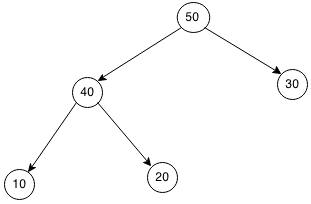
\includegraphics[scale=0.5]{images/28_1_3.png}
				\vspace{0.5cm}
		\end{enumerate}
	
	\item[2.] Trace the addition of each of the following values to an initially empty maxheap:
		
		\vspace{0.1cm}
		10 20 30 40 50
		
		\vspace{0.1cm}
		Compare your trace with the results of Exercise 1a.
		\begin{itemize}
			\item This question asks you to trace the creation of the heap if each node is added one at a time (instead of adding all of the nodes and restructuring - like you did in \#1). Show the tree only for each step (you do not need to show the array). You will show what the tree looks like when a new node is added and you will show what the tree looks like when reheap is called as a result of each addition.
		\end{itemize}
		
		\vspace{0.5cm}
		add 10
		
		\vspace{0.5cm}
		
\includegraphics[scale=0.5]{images/28_2_1.png}
		
		\vspace{0.5cm}
		add 20
		
		\vspace{0.5cm}
		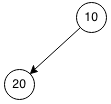
\includegraphics[scale=0.5]{images/28_2_2.png}
		
		\vspace{0.5cm}
		reheap(1)
		
		\vspace{0.5cm}
		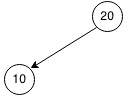
\includegraphics[scale=0.5]{images/28_2_3.png}
		
		\vspace{0.5cm}
		add 30
		
		\vspace{0.5cm}
		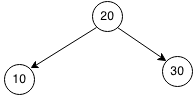
\includegraphics[scale=0.5]{images/28_2_4.png}
		
		\vspace{0.5cm}
		reheap(1)

		\vspace{0.5cm}
		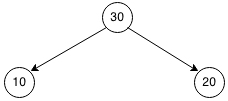
\includegraphics[scale=0.5]{images/28_2_5.png}
		
		\vspace{0.5cm}
		add 40
		
		\vspace{0.5cm}
		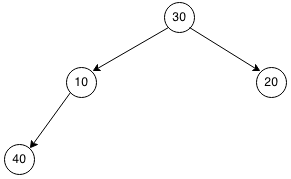
\includegraphics[scale=0.5]{images/28_2_6.png}
		
		\vspace{0.5cm}
		reheap(2)
		
		\vspace{0.5cm}
		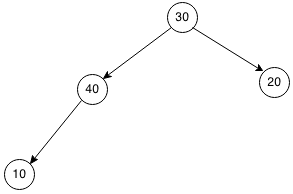
\includegraphics[scale=0.5]{images/28_2_7.png}
		
		\vspace{0.5cm}
		reheap(1)
		
		\vspace{0.5cm}
		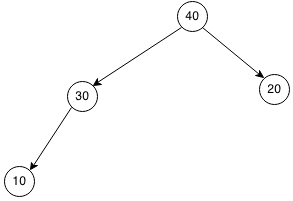
\includegraphics[scale=0.5]{images/28_2_8.png}
		
		\vspace{0.5cm}
		add 50
		
		\vspace{0.5cm}
		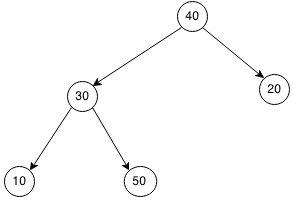
\includegraphics[scale=0.5]{images/28_2_9.png}
		
		\vspace{0.5cm}
		reheap(2)
		
		\vspace{0.5cm}
		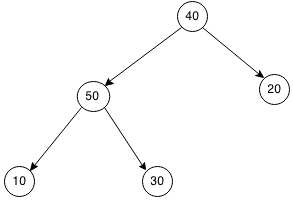
\includegraphics[scale=0.5]{images/28_2_10.png}
		
		\vspace{0.5cm}
		reheap(1)
		
		\vspace{0.5cm}
		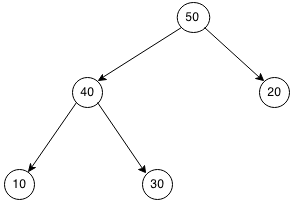
\includegraphics[scale=0.5]{images/28_2_11.png}
		\vspace{0.5cm}
\end{enumerate}

\end{document}